\documentclass[letterpaper]{article}
%\usepackage{../../../LaTeX/styles/aaai}
\usepackage{aaai}
\usepackage{times}
\usepackage{helvet}
\usepackage{courier}
\usepackage{latexsym} 
\usepackage{graphicx}
\usepackage{algorithm}
\usepackage{algorithmic}
\usepackage{url}
\usepackage{colortbl}
\usepackage{color}
\usepackage{subfigure}
\usepackage{amsmath}
\usepackage{amssymb}

\newtheorem{df}{Definition}
\newtheorem{notation}{Notation}
\newtheorem{theorem}{Theorem}[section]
\newtheorem{lemma}{Lemma}[section]
\newtheorem{col}{Corollary}
\newcommand{\bt}{\begin{theorem}\em}
\newcommand{\et}{\end{theorem}}
\newcommand{\Qed}{$\blacksquare$}
\newcommand{\qed}{$\Box$}
\newcommand{\proof}{{\bf Proof. }}

\newcommand{\nin}{\noindent}

\newcommand{\bea}{\begin{eqnarray}}
\newcommand{\eea}{\end{eqnarray}}

\newcommand{\bdf}{\begin{df}\em}
\newcommand{\edf}{\end{df}}

\newcommand{\ben}{\begin{enumerate}}
\newcommand{\een}{\end{enumerate}}
\newcommand{\ie}{\item}

\newcommand{\dist}{\operatorname{dist}}

\newcommand{\avg}{\operatorname{avg}}

\definecolor{grey}{rgb}{0.4,0.4,0.4}


\numberwithin{equation}{section}
\numberwithin{theorem}{section}
\numberwithin{lemma}{section}
\numberwithin{df}{section}

\title{Strategies for Multi-Player Drafting Games and Their Application to Risk}

\nocopyright

\author{Neesha Dessai, Richard Gibson \and Richard Zhao \\
Department of Computing Science, University of Alberta \\
Edmonton, Alberta, T6G 2E8, Canada \\
$\{$neesha$\mid$rggibson$\mid$rxzhao$\}$@cs.ualberta.ca}


\begin{document}

\maketitle

\begin{abstract}
A \emph{drafting game} is a game played by a set of $n$ players, where items are picked in turn without replacement from a communal collection.  Players attempt to maximize an individual end-game reward based on the unordered sets of choices made by each of the players.  A drafting game could stand alone, or it could be a sub-game of a larger, encompassing competition.  We investigate several approaches to playing drafting games including a new, novel strategy called the KthBestPick algorithm.  In addition, we show how to apply machine learning to guide these approaches when the players' objectives are not clear in the drafting game, but are realized in an encompassing game.  We test our techniques in the standard version of the board game Risk, where play begins with players picking territories in turn.  We find that UCT and KthBestPick yield the strongest drafting strategies in a game we call ``Fantasy Risk.''  Furthermore, we augment an existing bot with a new drafting strategy to create a program which outperforms the strongest opponents supplied with the computer game Lux Delux, a clone of the board game Risk.
\end{abstract}

\section{Introduction}

% Talk about search for single agent, minimax for two-player, 0-sum, MaxN for multi-player.  Examples like chess, checkers, etc.

For at least the past few decades, games have been an exceptional platform for artificial intelligence research.  Many successful computer programs have been developed which play at expert levels in two-player games such as Othello \cite{Othello}, checkers \cite{Chinook}, chess \cite{DeepBlue}, and Go \cite{ComputerGo}.  These games can be handled reasonably well by classic and modern artificial intelligence techniques, such as minimax search and Monte-Carlo tree search.  However, multi-player (i.e., more than 2 players) games are less understood.  In this paper, we explore strategies for playing multi-player ``drafting'' games.  Informally, a drafting game involves players taking turns selecting from a collection of items without replacement until some end game condition has been met.  At the conclusion of the game, each player receives an individual reward based on who chose which items; the order of the selections is irrelevant.  The objective for each player is to maximize her individual end game reward.  Some challenges associated with drafting games are dealing with large action spaces and considering how the choices of other agents should effect our own.

% Also include Risk in this discussion
There are a number of games, including both traditional board games and modern commercial video games, which either can be modelled as a drafting game or incorporate some kind of draft within part of the game.  A simple example is Tic-Tac-Toe, where two players take turns picking cells of a 3-by-3 grid until one player forms a line of 3 cells in a row with his picks (a win) or all cells are claimed (a draw).  Here, we can consider the player in the winning position at game's end receiving a positive reward while the losing player receives a negative reward, whereas zero reward is received in drawn endings.  Another example is the board game Risk by Hasbro Inc., which begins by players drafting the territories on the board until every territory has an owner.  Drafting territories in Risk presents an additional challenge as it is not clear what selections are best to make in order to eventually win the overall game.  

As for video games, sports simulations in particular often include a drafting aspect.  For instance, when playing through multiple seasons of the baseball game \textit{MLB 09: The Show} from Sony, a rookie draft takes place in between each season, where the human player and the computer opponents take turns choosing from a pool of new players who may then be added to the respective team's roster.  Another example is the new hockey game \textit{NHL 10} by EA Sports, where a fantasy draft can be activated at the beginning of a season.  In a fantasy draft, all players are removed from their current teams, and then selected one-by-one by the agents (human or computer-controlled teams) in the league.  Like with Risk, it is hard to judge which selections will improve a team's chance of winning the most.  Finally, the video game \textit{Star Wars: Empire at War} contains a drafting-type game where one can choose their ground force composition, execute ``auto-combat,'' and see the outcome of the battle.

Our main contributions in this paper are the following:
\begin{itemize}
	\item a novel adversarial search algorithm, KthBestPick, specifically designed for playing drafting games;
	\item a method for evaluating the opening draft in Risk using supervised maching learning; and
	\item a Risk bot, derived from an existing program but augmented with a new drafting strategy, which outperforms a number of difficult opponents.
\end{itemize}
The rest of the paper is organized as follows.  First, we formally describe drafting games and explain the potential need to create our own reward signal for some games.  We then discuss related work, followed by an introduction to the drafting strategies we try in Risk.  Next, we outline the basic rules of Risk and show how we apply supervised machine learning to generate a reward signal for the opening draft in Risk.  Finally, we empirically test our algorithms in Risk games, discuss the results, and conclude with some future works.

\section{Problem Formulation}
\label{sec:Prob}

Below, we formalize the concept of a drafting game and discuss the problems we explore associated with such a game.

\subsection{Drafting games}
\label{subsec:DraftingGames}

A \emph{drafting game} is a finite, deterministic, full-information game played by a set of $n \geq 2$ players, which we label 1 through $n$.  The game has a single set of actions or \emph{picks} $A$ initially available to every player.  Once a player makes a pick, that pick is forbidden to all players for the rest of the game.  Play continues until some predefined end game condition is satisfied or all actions in $A$ have been chosen.  At the game's conclusion, the picks made by each of the players induce a partition $Z = \{A_1, ..., A_{n}, \bar{A}\}$ of $A$, where $A_i$ is the set of all picks made by player $i$, and $\bar{A}$ are the actions that were not chosen by any player.  Each player then receives a reward signal $r_i(Z)$ according to the resulting partition $Z$.  Player $i$'s objective is to make picks in such a way as to maximize $r_i(Z)$.  Note that this means there is not necessarily a single winner; players may be following their own individual and independent objectives.

\subsection{Engineering the reward signal}

Some drafting games, like Tic-Tac-Toe, are stand-alone games which naturally inherit a reward signal from the rules and objectives of the game; for example, the reward signal
\[ r_i(Z) = \left\{ \begin{array}{cl} 1 & \text{if player $i$ has 3 cells in a row in $Z$,} \\ -1 & \text{if the other player has 3 cells in a row in $Z$,} \\ 0 & \text{otherwise} \end{array} \right. \]
acts as a clear objective for player $i$ to maximize in Tic-Tac-Toe.  However, in many applications, a drafting game is a precursor to a larger competition involving the same set of players.  For example, in Risk, once players draft territories, the game continues until a single player wins by occupying all territories on the map.  If we want to consider the opening draft as its own separate sub-game, it is not immediately clear what the reward signals should be.  For such a sub-game, the task is thus to create a reward signal $r_i(Z)$ for each player in the drafting game that correlates with the objectives of each player in the encompassing game.  Throughout this paper, we refer to these drafting games as ``drafting sub-games.''

\section{Related Work}

Perhaps the most widely known approach to computer game playing is the minimax adversarial search algorithm.  It is designed for zero sum games involving two players, denoted Max and Min.  The Max player (assumed to be the active player) performs a search of a game tree rooted at the current state of the game.  Each leaf node of the tree is evaluated by a heuristic function, which returns a value estimating the merit of the state to Max.  These values are then backed up the tree; at nodes belonging to Max, the maximum value of all child nodes is propagated up, whereas at nodes belonging to Min, the minimum value of the children is backed up.  The Max player then chooses the action leading to the child with the maximum propagated value.

% MaxN, Paranoid
% MP-Mix which extends MaxN (was used only for branching factor of 3, and for single winner games)

While minimax search is a traditional strategy employed in many two-player games, it is not applicable to games with $n > 2$ players.  Perhaps the simplest generalization of traditional minimax search to more players is the MaxN algorithm \cite{MaxN}.  At the leaf nodes of the game tree, a heuristic function now estimates a vector of $n$ merits $(h_1, ..., h_n)$, one for each player.  At nodes belonging to player $i$, the vector with the highest merit $h_i$ is propagated up to the parent.  Thus, players are assumed to be maximizing their own individual payoffs throughout the remainder of the game.  An alternative to MaxN is the Paranoid algorithm \cite{Paranoid}, where the active player assumes that the other players are out to minimize her payoff with complete disregard to their own benefits.  The Paranoid algorithm is essentially equivalent to the minimax algorithm, where the other players are represented as one meta-player (Min) attempting to minimize the individual heuristic value of the active player (Max).  Finally, the MaxN and Paranoid propagation strategies can be dynamically selected according to the game situation.  This is done in the MP-Mix algorithm \cite{ZuckFelnerKraus2009}, along with a third strategy called Offensive.  However, MP-Mix was designed for games with only a single winner, which does not directly fit into our general framework of a drafting game.  On the whole, each of these algorithms perform best when the branching factor (i.e.~action space) is small and when there exists a good evaluation function for approximating the merits of non-terminal states.  In general, drafting games can have a very large branching factor.  We also know of no such evaluation function for the drafting sub-game of Risk.

% Meta-models for reducing action space

Finally, Lee's work is closely related to drafting sub-games.  In his thesis \cite{GregLeeThesis}, Lee combines heuristic search with a machine-learned fitness function to pick a set of actions from a large library, which an agent is then restricted to in a Markov Decision Process.  The objective is to find a small set of actions which enable the agent to behave as close to optimal as possible in its domain, relative to having access to the entire library of actions.  Our work with drafting sub-games can be seen as an extension of Lee's work from a single-agent problem to a competitive multi-agent problem, where we replace heuristic search with adversarial methods. 

\section{Drafting Game Strategies}
\label{sec:drafting}

We investigate three different approaches to playing drafting games: Reinforcement learning (RL), UCT, and a novel adversarial search algorithm for drafting games, KthBestPick.  We now discuss each of these below.

\subsection{Reinforcement Learning}

% Describe reinforcement learning in general and how we applied it to drafting games.
Reinforcement learning is a machine learning technique where a learning agent takes actions in an environment with the goal of maximizing long-term reward.  A frequently applied reinforcement learning algorithm is Sarsa($\lambda$) \cite{SuttonBarto1998}.  In Sarsa($\lambda$), an agent maintains a set of states representing the environment and a set of valid actions the agent can take in the environment. Time is divided into discrete steps and one action is taken at each step.  At each step, a reward \textit{r} is calculated from observations of the environment.   To choose an action at each step, a policy is used.  A policy $\pi$ is a mapping of each state \textit{s} and each action \textit{a} to the probability of taking \textit{a} in \textit{s}.  The value function for $\pi$, denoted Q(s,a), is the expected total future reward of taking \textit{a} in \textit{s} and following $\pi$ to the end.  At each step, the Q function is updated by a temporal-difference error based on the reward received.
When the $\lambda$ parameter has value 0, only the Q values associated with the last action performed receive an update. However, when $\lambda$ is strictly between 0 and 1, the sequence of actions performed until the current step receives an update.  The update received is multiplied by e, the eligibility trace, which is in turn discounted by a factor $\lambda$, according to the following:

\[ Q(s_t, a_t) = Q(s_t, a_t) + {\alpha} {\delta} e(s_t, a_t) \]
\[ where \ {\delta} = r_{t+1} + \\ {\gamma}Q(s_{t+1}, a_{t+1}) - Q(s_t, a_t) \]

In the game of Risk drafting, actions need to be abstracted, since making an action from selected each territory would mean that there are 42 actions to choose from, and learning to differentiate between all actions would take an infeasible amount of time.  The eight abstracted actions used in the experiments are: choose the most empty continent; choose the least empty continent; choose the continent with the most number of my territories; choose the continent with the least number of my territories; choose the smallest available continent; choose the largest available continent; choose the continent with the most access points (links to other continents); choose the continent with the least access points.  Four binary state variables representing the environment are used: I am the sole owner of a continent; I have more than half of all territories in a continent; an opponent has more than half of all territories in a continent; there is an empty continent.  Once an action is chosen, an action resolution mechanism is invoked to pick a territory within the chosen continent, based on the strategy that having territories close to one another is better than having territories separated by enemies.
From some preliminary experiments, it is determined that the following parameters produced the best results: $\alpha$ (learning rate) = 0.1, $\epsilon$ (exploration rate) = 0.2, $\gamma$ (discount factor) = 1.0, $\lambda$ = 0.9.  These are the values used in subsequent experiments.

% Any theoretical properties to mention?
\subsection{Theoretical Analysis}

The Sarsa($\lambda$) algorithm, with a decreasing exploration rate, has the property that it converges with probability 1 to an optimal policy and value function as long as all state-action pairs are visited an infinite number of times, and the policy converges to a greedy policy  \cite{SuttonBarto1998}.  In the Risk implementation, this property is satisfied with an $\epsilon$-greedy policy, where $\epsilon =$ 0.2 / max (1.0, t/100), and t is the time step.  This algorithm will converge to an optimal policy with respect to the action abstraction as time step goes to infinity. 


\subsection{UCT}

UCT is a Monte Carlo planning algorithm that was first presented by~\cite{UCT}. UCT tries to intelligently bias the game tree as it's building it to focus on appealing branches and further search those. At each step, in our case time to pick the next territory, UCT builds upon the sparse game tree from the previous iterations by selecting branches to expand according to the formula

\[ Q(s,a)_{new} = Q(s,a)_{old} + c* \sqrt{\frac{log n(s)}{n(s,a)}}, \]

where $Q(s,a)$ is the value at the current node, $c$ is a exploration  constant, $n(s)$ is the number of times the node has been visited and  $n(s,a)$ is the number of times each action has been explored. $Q(s,a) $ is an $n$-tuple of the average reward signal vector $r(Z)$ seen on  all simulations through $s$ where action $a$ was taken.  On each  rollout, UCT adds one new node to the game tree and then uses Monte  Carlo rollout to determine the rest of the game from that node. The $n $-tuple of values it returns (one value per player) are they  propagated up the tree.  If UCT was allowed to perform an infinite  number of rollouts and the exploration constant was infinitely high,  UCT would become strictly Monte Carlo planning. UCT requires two  pieces of information from the user, $x$ and $c$ where $x$ is the  number of rollouts to perform at each step and $c$ is the exploration  constant. For our paper, we refer to our iterations of UCT as UCT($x$,  $c$).

For multiplayer UCT, each node stores an $n$-tuple of values, one for each player. When player $i$ is to choose the next branch to expand, the formula maximizes the $i$th value from the $n$-tuples of the children. Multiplayer UCT has most commonly been used in general game playing, for example in CadiaPlayer by~\cite{Cadia}. 


% Describe UCT, specifically for multi-player games (like drafting games)

% May want to discuss theoretical properties of UCT (converges to Nash equilibrium?)

% Perhaps mention UCT being used in GGP (plus reference)?

%Monte-Carlo tree search algorithms, such as UCT \cite{UCT}, are a different approach to game playing than minimax-type methods.  Simply put, thousands of games are simulated to completion, and each node's value is set to the average of the outcomes which passed through that node.  As game tree sizes typically grow exponentially in their branching factor, minimax-type algorithms must often rely on an accurate heuristic function at non-terminal nodes due to memory or time constraints.  Monte-Carlo tree search, on the other hand, needs no heuristic function and receives an unbiased estimate of the value of each action.  Because of this, UCT is often preferred in games with large action spaces or which lack a quality heuristic function, and has had much success in Computer Go \cite{ComputerGo}.  As drafting games typically have large, initial action spaces and lack a general heurstic function, we have implemented UCT as a drafting strategy.  UCT is also used as a base for our new algorithm, KthBestPick (see Section \ref{sec:KthBestPick}).

\subsection{The KthBestPick Algorithm}
\label{sec:KthBestPick}
% kthBestPick search

While both RL and UCT can be applied to many different domains, the KthBestPick algorithm focuses specifically on drafting games.  The idea here is that it may not always be best to pick the action which improves our situation the most.  For instance, suppose we are considering two particular actions, A and B, that will both benefit our end-game reward.  Suppose further that we know picking B will be slightly more beneficial to us than picking A.  If no other player will benefit themselves from picking B, but a player will benefit from picking A, then we should consider picking A now with our current action, as it seems likely that B will be available with our next pick.  If we choose B now, A may not be available on our next turn.  At each turn, KthBestPick uses a heuristic function to rank the available picks from best (rank 0) to worst (rank equal to the number of picks remaining minus 1).  Then, it estimates the most inferior pick of rank $k$ that we may choose so that we eventually pick all $k$ better-ranked actions (rank 0, 1, ..., $k-1$) with our later picks.  This is done using opponent models to predict the play of the other players, which may or may not be different from the heuristic function.

\begin{algorithm}[t]
	\caption{KthBestPick($node$, $h$, $m_0$, ..., $m_{n-1}$)}
	\label{alg:kth}
	\begin{footnotesize}
	\begin{algorithmic}[1]
		\STATE $rankedPicks \gets $ sort($node$.getActions(), $h$)
		\STATE $p \gets node$.getActivePlayer()
		\FOR{$k$ from $node$.getNumPicksLeft(p)$-1$ to $0$}
			\STATE $pick \gets rankedPicks(k)$
			\STATE $betterPicks \gets rankedPicks(0..k-1)$
			\STATE $child \gets node.$getChild($pick$)
			\STATE $makeThisPick \gets $ TRUE
			\WHILE{$betterPicks$ is not empty}
				\IF{$child$.isGameOver()}
					\STATE $makeThisPick \gets $ FALSE
					\STATE BREAK
				\ENDIF
				\STATE $p \gets child$.getActivePlayer()
				\STATE $nextPick \gets m_p(child)$
				\STATE $child \gets child.$getChild($nextPick$)
				\IF{$nextPick \in betterPicks$}
					\IF{$p = node$.getActivePlayer()}
						\STATE $betterPicks.$remove($nextPick$)
					\ELSE
						\STATE $makeThisPick \gets $ FALSE
						\STATE BREAK
					\ENDIF
				\ENDIF
			\ENDWHILE
			\IF{$makeThisPick$}
				\RETURN{$pick$}
			\ENDIF
		\ENDFOR
	\end{algorithmic}
	\end{footnotesize}
\end{algorithm}

Algorithm \ref{alg:kth} gives the pseudocode for KthBestPick, which takes in the current state $node$, a heuristic function $h$, and a sequence of opponent models $m_0, ..., m_{n-1}$ (one for each player) as parameters.  We first rank the actions according to the heuristic function (line 1) according to the merit of the picks in the active player's perspective.  Next, $k$ is set to one less than the number of picks remaining for the active player (line 3), as we do not have enough picks to consider more inferior actions.  Then, we set our potential pick to the action ranked $k$ (line 4), construct a list containing all of the superior picks (line 5), and initialize $child$ to point to the child node associated with this potential pick.  To determine if this pick is desired, we repeatedly find each of the next picks made by the players according to the opponent models (line 14).  Each model returns the action believed to be picked by the active player at the passed in node.  After updating our $child$ pointer to follow this next pick (line 15), we check if the pick is in our list of superior actions (line 16).  If it is, there are two possible cases.  If the pick was made by caller of the algorithm (line 17), then this is allowed; we remove the pick from the superior list (line 18) and continue.  However, if the pick was made by another player, then we abandon our potential pick (lines 20 and 21), decrement $k$ (line 3), and now consider the new potential pick ranked $k$ (line 4 again).  If the list of superior picks ever becomes empty (line 8), this indicates that the original active player is predicted to pick all of the superior actions, and so we return the current potential pick (line 26).  However, if the game ends while superior actions remain unclaimed (line 9), we instead abandon the potential pick (lines 10 and 11). 

% Possible heuristic functions: learn one based on a number of features describing the current state-action space, or can use MaxN-MC.
There are a number of different possibilities for the heuristic function.  The most obvious choices are one of our other two drafting strategies, RL or UCT.  Both of these techniques store a value for each available action estimating the merit of making that pick, allowing the actions to be sorted as necessary.

% Possible opponent models: KthBestPick (in practice, keep track of repeated calls in one state, and truncate the game to a fixed maximum number of picks remaining), if repeated games then could try to learn an opponent model.  Typically will not be given the explicit opponent drafting strategies.
As for the opponent models, again there are a few options.  Firstly, we should use KthBestPick as the opponent model for our own play, since we know this is the strategy being used to make our picks.  Typically for the other players, however, we will not be given their explicit drafting strategies.  The simplest approach would be to assume that the opponents are also using KthBestPick to make decisions with an appropriate self-centered heuristic function.  This turns line 14 of Algorithm \ref{alg:kth} into a recursive call, and in this case, KthBestPick can be very costly in computation time.  We can combat this by only considering a fixed number of the highest ranked picks at line 3, and repeating the algorithm iteratively on this number until returning a pick is necessary.  Finally, if we are fortunate enough to have obtained the strategies of our opponents, we can simply pass these into the algorithm.

We now consider a small example to build up intuition behind the KthBestPick algorithm.  Consider the drafting game with four actions, A, B, C, and D, and three players, 1, 2, and 3.  Players pick in numerical order until all actions have been picked (thus player 1 gets two picks).  For each action and each player, we associate a point value that that player receives for making that pick.  A player's reward at the end of the game is simply the sum of the points of his picks.  Suppose the point values are as given in Table \ref{tab:KthEx}, and let's assume that we are player 1.  If we rank picks according to the point values for us only, then B would appear to be the best pick (4 points) and A the second best (3 points).  Following this heuristic alone would have us pick B.  Now if players 2 and 3 are playing optimally, player 2 will follow by picking A, then player 3 will pick C.  This forces us to pick D, leaving us with a reward of $4 + 1 = 5$.  However, if we apply KthBestPick with this heuristic and assume our opponents play optimally, then we will see that picking A first will lead player 2 to pick D and player 3 to pick C, leaving us to pick B with our last pick.  In this case, we end the game with a reward of $3 + 4 = 7$, a better result.  Note that UCT will also conclude that picking A first is a better move, but only after a number of simulations.  KthBestPick, on the other hand, finds the solution with just one ``simulation.'' 

\begin{table}[t]
	\begin{center}
		\caption{The point values for an example drafting game.}
		\label{tab:KthEx}
		\begin{footnotesize}
		\begin{tabular}{|c|c|c|c|c|}
			\hline
			\bf Player $\backslash$ Action & \bf A & \bf B & \bf C & \bf D \\
			\hline
			\bf 1 & 3 & 4 & 2 & 1 \\
			\hline
			\bf 2 & 4 & 1 & 2 & 3 \\
			\hline
			\bf 3 & 4 & 2 & 3 & 1 \\
			\hline
		\end{tabular}
		\end{footnotesize}
	\end{center}
\end{table}

\section{Theoretical Analysis}

\begin{theorem}
	\label{thm:Kth}
	KthBestPick always returns an action.
\end{theorem}
\begin{proof}
Firstly, the while loop in Algorithm \ref{alg:kth} (line 8) is not infinite.  This is because drafting games are finite and acyclic (no state can be repeated), and each pass through the loop makes one more action.  Thus the condition at line 9 must eventually be met.  Now consider the value of $k$ in the for loop at line 3.  If $k = 0$, then the $betterPicks$ list is set to empty (line 5), implying that the while loop condition (line 8) is false  and we return our pick (line 26).
\end{proof}

\section{Risk}

We use Risk as a testbed for our proposed drafting approaches.  Risk is a strategy board game for two to six players where the objective of the game is to occupy all 42 territories on the board.  The territories are divided into 6 continents, with 4 territories in both Australia and South America, 6 in Africa, 9 in North America, 7 in Europe, and 12 in Asia.  Figure \ref{fig:Conts} depicts their arrangement on the board.  In the standard rules, players first take turns selecting the territories until all have been chosen (the drafting sub-game).  After each player places their initial armies among their selected territories, players then take turns until only one player remains.  On a turn, in sequence a player may place reinforcements, conduct attacks on opposing territories, and tactically maneuver armies amongst owned territories.  Attacks are resolved by dice rolls, where the number of dice is dependent on the number of attacking and defending armies.  A player reduced to zero armies on the board is eliminated from the game.  Players receive one reinforcement army for every three territories owned and receive bonus reinforcements for owning entire continents or trading in cards earned by conquering territories.  Each continent has its own reinforcement bonus as depicted in Figure \ref{fig:Conts}.  Full rules can be found on-line\footnote{\url{http://www.hasbro.com/common/instruct/Risk.pdf}}.

\begin{figure}[t]
	\centering
	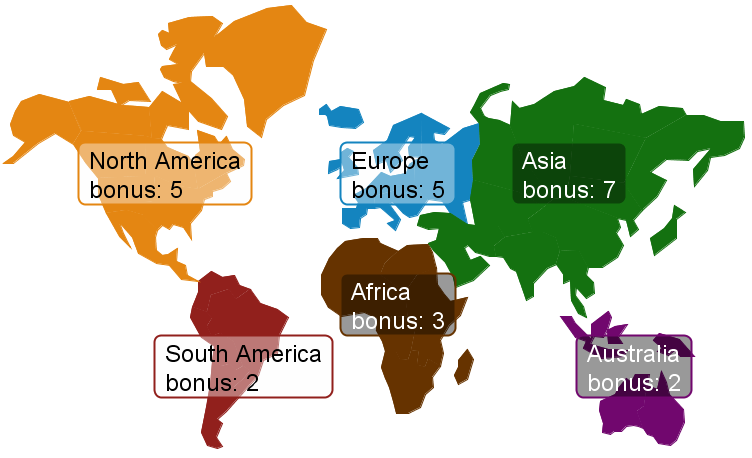
\includegraphics[scale=0.325]{figs/Conts.png}
	\caption{The layout of the Risk board and the continent reinforcement bonuses.}
	\label{fig:Conts}
\end{figure}

The Lux Delux\footnote{\url{http://sillysoft.net/lux/}} game provides a computer version of Risk, along with several AI bots (with source code) to play against, all of which are rule-based.  Each of the included bots has an associated difficulty and a general playing style.  For example, ``Quo'' is a difficult bot which tries to form a cluster of adjacent territories and methodically expand that cluster.  We use the Lux Delux environment in all of our computations and experiments.

In this paper, we are only concerned with strategies for playing the drafting sub-game at the beginning of Risk.  Strategies for the other phases of Risk are interesting and have been researched (\cite{RiskBots}, \cite{ZuckFelnerKraus2009}), but we do not investigate these here.  In addition, we decided to focus only on three player Risk, as this incorporates the multi-player aspect of drafting games and is arguably more strategically demanding compared to playing with more players.  This is because each player must make more selections per draft.

\section{A Machine-Learned Reward Signal}

Our objectives in this paper include both determining what strategies are desirable in drafting games, and finding a strategy in the Risk drafting sub-game that can improve our chances of winning in the full game of Risk.  The latter problem suffers from a few complications.  First, the merit of a strategy for the drafting sub-game may highly depend on the strategy used in post-draft play.  For instance, a drafting strategy that primarily selects territories in North America would not be advisable to play with a post-draft strategy that plays to own Australia at all costs.  With this post-draft strategy, it would make more sense to simply select territories in Australia rather than North America during the draft.  Secondly, as mentioned previously, it is not easy to classify a draft outcome $Z$ as either ``good'' or ``bad'' for player $i$.  This makes it difficult to guide drafting selections towards desirable outcomes.  What we are lacking is a reward signal $r_i(Z)$ that approximates player $i$'s chances of winning from $Z$ when following a given post-draft strategy.  In this section, we describe how we used supervised machine learning to create such a reward signal.

We identified a number of features that are tactically important in Risk.  Many of these features are inspired by those found in the evaluation function described in \cite{RiskBots}.  For each player, our features are described by:
\begin{itemize}
	\item[(i)] for each continent, the number of territories owned in that continent;
	\item[(ii)] when the player plays in the turn order;
	\item[(iii)] the number of distinct territories owned by other players which border owned territories (enemy neighbours); and
	\item[(iv)] the number of distinct ordered pairs of owned territories which are adjacent (friendly neighbours).
\end{itemize}
The merit of each feature set is estimated by a process similar to how Lee creates a domain-specific fitness function or meta-model for selecting a set of actions in a Markov decision process \cite{GregLeeThesis}.  Our process is depicted in Figure \ref{fig:MachLearn}.  First, we collect several draft outcomes, each obtained by randomly assigning all 42 territories evenly among the three players.  Then, for each draft outcome, 100 games are played to completion where each player follows the post-draft strategy of the Quo bot (see Risk section).  Each player $i$, $i=1,2,3$, has a set of features $S_i$ associated with each outcome.  Each feature set is assigned a value $v_i \in \{0,1,...,100\}$ equal to the number of games that player $i$ eventually won from the associated draft outcome.  This provides a collection of feature set value pairs $\{(S_i, v_i)\}$ of size equal to three times the number of draft outcomes collected.  Next, supervised machine learning is applied to obtain a general function
\[ f: S \mapsto v \in \textbf{R} \] 
that estimates the merit of the feature set $S$ when following Quo's post-draft strategy.  Finally, for a draft outcome $Z = (A_1,A_2,A_3,\phi)$, we calculate $v_i = f(S_i)$ where $S_i$ is the feature set associated with $A_i$, and define the reward signal for player $i$ to be
\[ r_i(Z) = \frac{v_i^+}{v_1^+ + v_2^+ + v_3^+}, \]
where $v_i^+ = \max(0, v_i)$.  Note that even though all training values $v_i$ are nonnegative, a learner could allow $f$ to be negative and so we take the max to keep the sign of $r_i(Z)$ correct.  Thus, to maximize reward, the objective of each player is to maximize the estimated merit of her selections while minimizing those of her opponents.

\begin{figure*}[t]
	\centering
	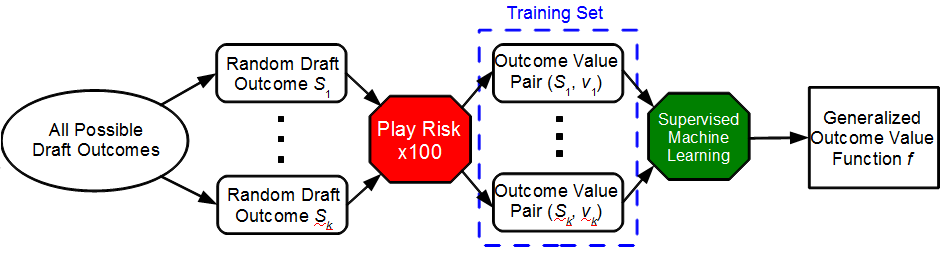
\includegraphics[scale=0.5]{figs/MachineLearner.png}
	\caption{The process described for obtaining a general function $f$ for estimating the merit of each feature set (adapted from \cite[Figure 5.1]{GregLeeThesis}).}
	\label{fig:MachLearn}
\end{figure*}

Our general function $f$ is computed from 7,364 random draft outcomes for a total of 22,092 $(S,v)$ pairs.  We use Weka \cite{Weka} to weight each individual feature using Weka's linear regression classifier (with no attribute selection), where features (i) and (ii) are represented as nominal features and features (iii) and (iv) are represented as numeric.  These weights are displayed in Tables \ref{tab:ContScoring} and \ref{tab:MoreScoring}.  However, there are some features which do not appear in any of the 22,092 feature sets because of their unlikeliness of occurring through random drafting; for instance, there were no cases where one player owned all 9 territories of North America.  The weights of these features are calculated through linear extrapolation of the closest two numbers in the continent counts for the associated continent.  For instance, the weight for owning all 9 territories in North America is calculated from the weights for owning 8 territories and 7 territories in North America via
\[ 36.1487 + (36.1487 - 24.0969) = 48.2005. \]  
Note that only in rare cases will $f$ be negative (lots of enemy neighbours and low scores elsewhere).  %SHOW DIAGRAM OF LINEAR EXTRAPOLATION FOR NORTH AMERICA?  ONLY IF THERE'S ROOM.

%\begin{table*}[t]
%  \begin{center} 
%   \caption{The weights for features of type (i), as computed in Weka.  A * denotes weights derived through linear extrapolation.}
%    \label{tab:ContScoring}
%    \begin{tabular}{|c|c|c|c|c|c|c|}
%    	\hline
%    	\bf Number of Territories & \bf Australia & \bf South America & \bf Africa & \bf North America & \bf Europe & \bf Asia \\
%    	\hline
%    	\bf 0 & 2.972 & 0.6904 & 14.3958 & 3.1092 & 42.4404 & 27.0974 \\
%    	\hline
%    	\bf 1 & 0 & 1.232 & 12.8728 & 0.9766 & 45.1071 & 23.9027 \\
%    	\hline
%    	\bf 2 & 8.4532 & 3.8997 & 10.7207 & 0 & 43.1116 & 23.6086 \\
%    	\hline
%    	\bf 3 & 9.9902 & 0 & 7.1637 & 2.1682 & 43.7726 & 23.1026 \\
%    	\hline
%    	\bf 4 & 10.7097 & 17.7184 & 1.23 & 7.1541 & 41.3515 & 23.6086 \\
%    	\hline
%    	\bf 5 & - & - & 0 & 19.3505 & 50.7666 & 23.6794 \\
%    	\hline
%    	\bf 6 & - & - & 29.796 & 24.8183 & 43.8472 & 19.3189 \\
%    	\hline
%    	\bf 7 & - & - & - & 24.0969 & 36.9278* & 15.6257 \\
%    	\hline
%    	\bf 8 & - & - & - & 36.1487 & - & 17.4338 \\
%    	\hline
%    	\bf 9 & - & - & - & 48.2005* & - & 13.8433 \\
%    	\hline
%    	\bf 10 & - & - & - & - & - & 10.2528* \\
%    	\hline
%    	\bf 11 & - & - & - & - & - & 6.6623* \\
%    	\hline
%    	\bf 12 & - & - & - & - & - & 3.0718* \\
%    	\hline
%    \end{tabular}
%  \end{center}
%\end{table*}

%\begin{table*}[t]
%  \begin{center} 
%   \caption{The weights for features of type (i), as computed in Weka.  A * denotes weights derived through linear extrapolation.}
%    \label{tab:ContScoring}
%    \begin{tiny}
%    \begin{tabular}{|c|c|c|c|c|c|c|c|c|c|c|c|c|c|}
%    	\hline
%    	  & \bf 0 & \bf 1 & \bf 2  & \bf 3 & \bf 4 & \bf 5 & \bf 6 & \bf 7 & \bf 8 & \bf 9 & \bf 10 & \bf 11 & \bf 12 \\
%    	 \hline
%    	\bf Australia & 2.972 & 0 & 8.4532 & 9.9902 & 10.7097 & - & - & - & - & - & - & - & - \\
%    	\hline
%    	\bf South America & 0.6904 & 1.232 & 3.8997 & 0 & 17.7184 & - & - & - & - & - & - & - & - \\
%    	\hline
%    	\bf Africa & 14.3958 & 12.8728 & 10.7207 & 7.1637 & 1.23 & 0 & 29.796 & - & - & - & - & - & - \\
%    	\hline
%    	\bf North America & 3.1092 & 0.9766 & 0 & 2.1682 & 7.1541 & 19.3505 & 24.8183 & 24.0969 & 36.1487 & 48.2005* & - & - & - \\
%    	\hline
%    	\bf Europe & 42.4404 & 45.1071 & 43.1116 & 43.7726 & 41.3515 & 50.7666 & 43.8472 & 36.9278* & - & - & - & - & - \\
%    	\hline
%    	\bf Asia & 27.0974 & 23.9027 & 23.6086 & 23.1026 & 23.6086 & 23.6794 & 19.3189 & 15.6257 & 17.4338 & 13.8433 & 10.2528* & 6.6623* & 3.0718* \\
%    	\hline
%    \end{tabular}
%    \end{tiny}
%  \end{center}
%\end{table*}

\begin{table*}[t]
  \begin{center} 
   \caption{The weights for features of type (i), as computed in Weka.  A * denotes weights derived through linear extrapolation.}
    \label{tab:ContScoring}
    \begin{footnotesize}
    \begin{tabular}{|c|c|c|c|c|c|c|c|c|c|c|c|c|c|}
    	\hline
    	  & \bf 0 & \bf 1 & \bf 2  & \bf 3 & \bf 4 & \bf 5 & \bf 6 & \bf 7 & \bf 8 & \bf 9 & \bf 10 & \bf 11 & \bf 12 \\
    	 \hline
    	\bf Australia & 2.97 & 0 & 8.45 & 9.99 & 10.71 & - & - & - & - & - & - & - & - \\
    	\hline
    	\bf South Amer. & 0.69 & 1.23 & 3.90 & 0 & 17.72 & - & - & - & - & - & - & - & - \\
    	\hline
    	\bf Africa & 14.40 & 12.87 & 10.72 & 7.16 & 1.23 & 0 & 29.80 & - & - & - & - & - & - \\
    	\hline
    	\bf North Amer. & 3.11 & 0.98 & 0 & 2.17 & 7.15 & 19.35 & 24.82 & 24.10 & 36.15 & 48.20* & - & - & - \\
    	\hline
    	\bf Europe & 42.44 & 45.11 & 43.11 & 43.77 & 41.35 & 50.77 & 43.85 & 36.93* & - & - & - & - & - \\
    	\hline
    	\bf Asia & 27.10 & 23.90 & 23.61 & 23.10 & 23.61 & 23.68 & 19.32 & 15.63 & 17.43 & 13.84 & 10.25* & 6.66* & 3.07* \\
    	\hline
    \end{tabular}
    \end{footnotesize}
  \end{center}
\end{table*}

\begin{table}[t]
	\begin{center}
		\caption{The weights for features (ii), (iii), and (iv) as computed in Weka.} 
		\label{tab:MoreScoring}
		\begin{footnotesize}
		\begin{tabular}{|c|c|}
			\hline
			\textbf{Feature} & \textbf{Points} \\
			\hline
			First to play & 13.38 \\
			\hline
			Second to play & 5.35 \\
			\hline
			Each unique enemy neighbour & -0.07 \\
			\hline
			Each ordered pair of friendly neighbours & 0.48 \\
			\hline
		\end{tabular}
		\end{footnotesize}
	\end{center}
\end{table}

We now show how to use Tables \ref{tab:ContScoring} and \ref{tab:MoreScoring} to compute $r_i(Z)$ for the draft outcome given in Figure \ref{fig:DraftExample}.  Player 1 (blue) has 4 territories in Australia, 0 in South America, 2 in Africa, 1 in North America, 3 in Europe, and 4 in Asia.  In addition, player 1 has 18 distinct enemy neighbours and 22 ordered pairs of friendly neighbours.  Assuming player 1 is first to play, $f(S_1)$ is computed as
\begin{eqnarray*}
% 	f(S_1) &=& [10.7097 + 0.6904 + 10.7207 \\ && +\ 0.9766 + 43.7726 + 23.6086] \\ &&+\ [13.3818 + 18(-0.0719) + 22(0.4799)] \\
% 				 &=& 113.124,
 	f(S_1) &=& [10.71 + 0.69 + 10.72 + 0.98 + 43.77 \\ &&+\ 23.61] + [13.38 + 18(-0.07) + 22(0.48)] \\
 				 &=& 113.12,
\end{eqnarray*}
where the values in the first set of brackets are from Table \ref{tab:ContScoring} and the second set of brackets are from Table \ref{tab:MoreScoring}.  We can similarly compute the values of the feature sets for player 2 (green) and player 3 (red) as %$f(S_2) = 89.4739$ and $f(S_3) = 119.6547$ 
$f(S_2) = 89.47$ and $f(S_3) = 119.65$ respectively, where player 2 is second to play.  Finally, $r_i(Z)$ is computed via
\[ r_i(Z) = \frac{f(S_i)}{f(S_1) + f(S_2) + f(S_3)}, \]
giving us %$r_i(Z) = \{0.3509, 0.2776, 0.3712\}$ 
$r_i(Z) = \{0.35, 0.28, 0.37\}$.

\begin{figure}[t]
	\centering
	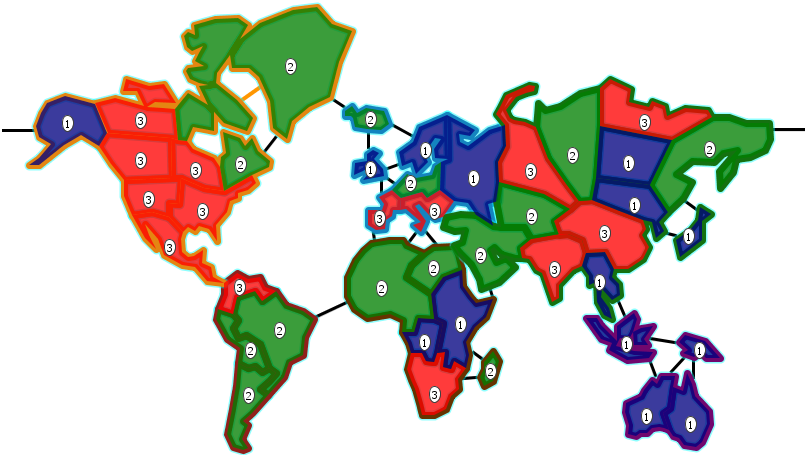
\includegraphics[scale=0.3]{figs/DraftExample.png}
	\caption{An example of a draft outcome.  The territories picked by players 1, 2, and 3 are blue, green, and red respectively.  Territories connected by a line are also considered adjacent or bordering.}
	\label{fig:DraftExample}
\end{figure}

\section{Empirical Evaluation}

In this section, we describe the drafting game we call ``Fantasy Risk,'' a stand-alone drafting game that mimics the drafting sub-game of standard Risk.  Then, we compare our drafting approaches in Fantasy Risk.  We end this section by combining UCT with Quo's post-draft strategy and facing off against the most difficult bots provided with Lux Delux.

\subsection{Fantasy Risk}

% Explain fantasy risk, plus give scoring table.
In Fantasy Risk, players take turns selecting from the 42 territories on the Risk board until all territories have been claimed, just as in the beginning of standard Risk.  Then, the game immediately ends and the players receive rewards according to the machine-learned reward signal described in the previous section.  Playing Fantasy Risk allows us to better analyze our different drafting strategies without worrying about the dynamics and variance of post-draft Risk.  

\subsection{Comparison of Algorithms in Fantasy Risk}

% Run experiments, graph results
In addition to our three proposed approaches, RL, UCT, and KthBestPick, we consider two baseline strategies.  The first is simply a player that picks territories at random.  The second, which we call ``GreedyDrafter,'' works as follows.  At any state $\hat{Z}$ in the draft (i.e.~a partial assignment of territories to players), we can obtain temporary feature sets $\hat{S_1}, \hat{S_2}, \hat{S_3}$ for each player of the current selections made, using the same features as described in the previous section.  We can then calculate the estimated reward signal $\hat{r}_i(\hat{Z}) = \frac{f(\hat{S_1})}{f(\hat{S_1}) + f(\hat{S_2}) + f(\hat{S_3})}$ of the state $\hat{Z}$.  GreedyDrafter picks the territory which leads to the state with the greatest estimated reward signal $\hat{r}_i(\hat{Z})$, breaking ties by selecting randomly among the territories with the fewest number of unoccupied neighbours.  For example, on an empty board, we can conclude from Table \ref{tab:ContScoring} that GreedyDrafter will always open with picking a territory in Europe with exactly three neighbours (the fewest of all territories in Europe).  GreedyDrafter can be seen as a 1-ply lookahead search that uses $\hat{r}_i(\hat{Z})$ as an evaluation function.

Figure \ref{fig:FantRisk1} compares RL and UCT$(3000, 0.01)$ against the two baseline strategies in Fantasy Risk.  Each of these results display the average rewards (multiplied by 100) received by each bot per game over 100 rounds, where one round consists of 6 games for each of the $3!$ turn orderings.  The vertical black bars indicate 95\% confidence intervals, measured per round and multiplied by $100 / 6$.  MENTION RL PARAMETERS AND SET UP HERE.  The UCT parameters were chosen for fast action selection (each took less than a second) and were found to perform well in preliminary experiments.  We can see in Figure \ref{fig:UCTvsRANvsGRE} that UCT outperforms the baselines by a large margin, approximately doubling the average rewards of GreedyDrafter.  In addition, Figure \ref{fig:UCTvsRLvsGRE} shows UCT on top again against RL and GreedyDrafter.  Note that our RL approach unfortunately fails in comparison to even the baseline GreedyDrafter strategy.

\begin{figure}[t]
\centering
\subfigure[]{
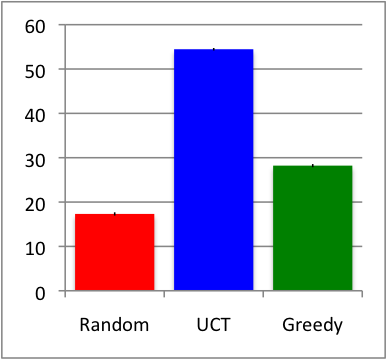
\includegraphics[scale=.55]{figs/random.png}
\label{fig:UCTvsRANvsGRE}
}\hspace{5pt}
\subfigure[]{
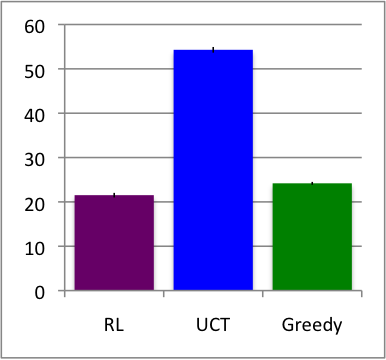
\includegraphics[scale=.55]{figs/rl.png}
\label{fig:UCTvsRLvsGRE}
}
\caption[]{Average Fantasy Risk rewards earned per game ($\times 100$) in contests featuring \subref{fig:UCTvsRANvsGRE}: Random vs.~UCT vs.~GreedyDrafter, and \subref{fig:UCTvsRLvsGRE}: RL vs.~UCT vs.~GreedyDrafter.}
\label{fig:FantRisk1}
\end{figure}  

Figure \ref{fig:FantRisk2} shows the results of two sets of 50 Fantasy Risk rounds of KthBestPick versus GreedyDrafter versus UCT$(\cdot, 0.01)$.  In both sets, KthBestPick uses UCT$(3000, 0.25)$ as its heuristic.  The exploration parameter was increased here since it is important for KthBestPick to not only have confidence about the highest ranked pick, but also to have confidence about the next best picks too.  For a fair comparison of KthBestPick and UCT, we instituted a time limit of 250 milliseconds per unowned territory on the board before a pick had to be made.  UCT simply ran as many simulations as possible in the time limit, while KthBestPick iterated on the number of lower-ranked picks considered in line 3 of Algorithm \ref{alg:kth}, returning the last selection made once time was up.  The iterations started by considering only the top ranked pick, meaning that the for loop (line 3) only executed once on the first iteration.  In addition, if the pick of rank $k$ was determined to be bad (line 10 or 20), we took the pick of rank $k-1$, simulated this move, and ran UCT simulations from the new state to improve future estimates of actions until time expired.  The UCT tree was only deleted from memory after each game.  Furthermore, we ran UCT simulations to rank the picks (line 1) only until at least 3000 simulations had been acquired from the current state, counting previous simulations through this node.  Finally, no program performed any ``thinking'' during another program's turn.

The average rewards shown in Figure \ref{fig:kthNoOrc} have KthBestPick using itself as the opponent model for all three players, whereas in Figure \ref{fig:KthOrc} KthBestPick uses UCT and the logic of GreedyDrafter to model its opponents appropriately.  We don't concern ourselves with how KthBestPick would obtain such models here, but only the benefits of having these ``oracles.''  The results of both cases are similar, as we can see KthBestPick beating UCT by a small margin.

\begin{figure}[t]
\centering
\subfigure[]{
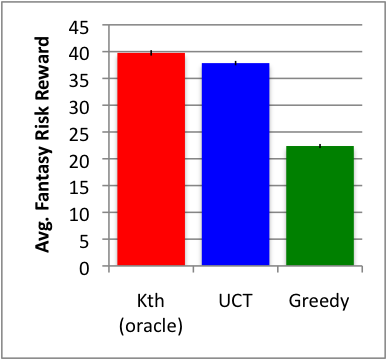
\includegraphics[scale=.55]{figs/kth.png}
\label{fig:kthNoOrc}
}\hspace{5pt}
\subfigure[]{
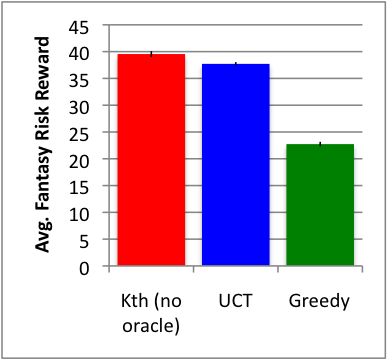
\includegraphics[scale=.55]{figs/kthno.png}
\label{fig:KthOrc}
}
\caption[]{Average Fantasy Risk rewards earned per game ($\times 100$) in contests featuring KthBestPick vs.~UCT vs.~GreedyDrafter.}
\label{fig:FantRisk2}
\end{figure}

%\subsection{Selfish Play}

% Run experiments, graph results

\subsection{Full Risk}

% Run experiments of actual Risk results and make graphs

We created a ``UCT-Quo'' bot for the full game of Risk by identically duplicating the rule-based strategy of the Quo bot, except replaced its drafting rules with our UCT$(3000,0.01)$ implementation guided by our machine-learned reward signal $r_i(Z)$.  We decided to use UCT rather than KthBestPick so that more games could be played, as KthBestPick requires more time per pick.  

We pitted our UCT-Quo bot against all four bots labeled as ``difficult'' in the Lux Delux game: Killbot, EvilPixie, Quo, and Boscoe.  Each subfigure of Figure \ref{fig:ActualRisk} reports the winning percentage of each bot over 100 rounds (again all 6 turn orderings played each round).  Figures \ref{fig:UCTvsQUOvsQUO}, \ref{fig:UCTvsQUOvsEP}, and \ref{fig:UCTvsKILvsBOS} show UCT-Quo winning significantly more than its fair share of games.  In particular, Figure \ref{fig:UCTvsQUOvsQUO} shows that when all players use Quo's post-draft play, a player drafting using UCT guided by $r_i(Z)$ wins frequently against two opponents that follow Quo's rule-based approach (which attempts to draft entire continents when possible).  However, Figure \ref{fig:UCTvsUCTvsQUO} shows that our bot is not perfect, as two UCT-Quo bots lose out to one Quo player.  

%All of our experiments will be conducted in the board game Risk using the Lux Delux\footnote{http://sillysoft.net/lux/} environment.  Lux Delux provides several Risk bots with source code, which include their own hand-coded drafting strategies.  Conveniently, this gives us plenty of competition to test our algorithms against.  We use the selected countries and placed initial armies options in all of our experiments.

%An evaluation function in Risk is provided by (Johansson \& Olsson 2006), and in more detail in (Olsson 2005), to calculate the value of a single territory.  This territory value is meant to approximate how desirable an enemy territory is to a player during gameplay.  The evaluation function is a sum of different sub-components, each measuring a unique situation in the game.  Advantageous situations are given positive values and disadvantageous situations are given negative values.  For example, it is desirable to have more friendly neighbours around a territory, thus the number of friendly neighbours to a territory is a sub-component that contribute positively to the value of this territory.
%We adopted this evaluation function to measure the value of an entire draft to a particular player.  The territory values given by the evaluation function for all territories owned by the player are added together, creating a draft evaluation function.  However, we have to make changes to Johansson \& Olsson's territory evaluation function (from here on referred to as JO) since some sub-components are not longer valid with our new intended purpose:
%\begin{itemize}
%  \item JO gives a value of 0.05 for each army in a friendly neighbour and -0.03 for each army in an enemy neighbour.  Since we are evaluating a complete draft before the post-draft play (where the placing of armies occur), these two components do not apply to us.
%  \item JO gives a value of 20 for owning the whole continent except this territory.  Thus this territory has a high value to the player.  Such a territory is highly desirable since obtaining an entire continent provides a bonus to armies.  In our case, we only give the same value for actually owning the whole continent, since in a final draft all territory ownerships are determined.
%  \item JO gives a value of 4 if an enemy owns the whole continent. In such cases, conquering this enemy territory is desirable since it prevents the enemy from getting the continent army bonus.  In our case, if an enemy owns a continent in the final draft, then it is disadvantageous for the player, so a value of -4 is given.
%\end{itemize}	
%	
%
%\subsection{Analyzing Evaluation Function}
%
%Before we committed to using the new evaluation function as we modified from the paper, we needed to test how well it worked at predicting completed draft states. To test this, we created 6 random draft configurations. These were created by having three agents randomly pick a territory, and then storing the values chosen by each so that they could be recreated later. Therefore, each draft configuration was made up of three sets of draft picks, one for each of the three players (agents). An example map is shown in Figure~\ref{fig:random}. We had a 7th draft configuration where one agent owns an entire continent, in this case Australia, which is shown in Figure~\ref{fig:continent}. 
%
%Next, we computed the evaluation function for each set of picks in each draft. From there, each draft was used to play two sets of 1000 games. The first 1000 games were played such that each agent chose their draft picks based on their turn order, so whichever agent went first on each game chose from set 0. The second set of 1000 games were played such that each agent always choose the same draft picks regardless of order, ie one agent always choose from set 0, one from set 1 and the third from set 2. The number of games each set won for each draft are presented in Table~\ref{tab:results}.
%
%The results show that there are draft combinations that the evaluation function is not taking advantage of, as show in the results for player 2 in set 1, or player 0 in set 2. The other interesting result is that for some draft selections, being the first player (as shown in the ordered results) can be an advantage, something we expected. But, there are cases where a draft set actually does better in the random configuration. By running more tests of the 6 possible orders for the three agents, we may be able to learn more about the advantages/disadvantages the turn order provides. 
%
%%\begin{figure}[htp]
%%\centering
%%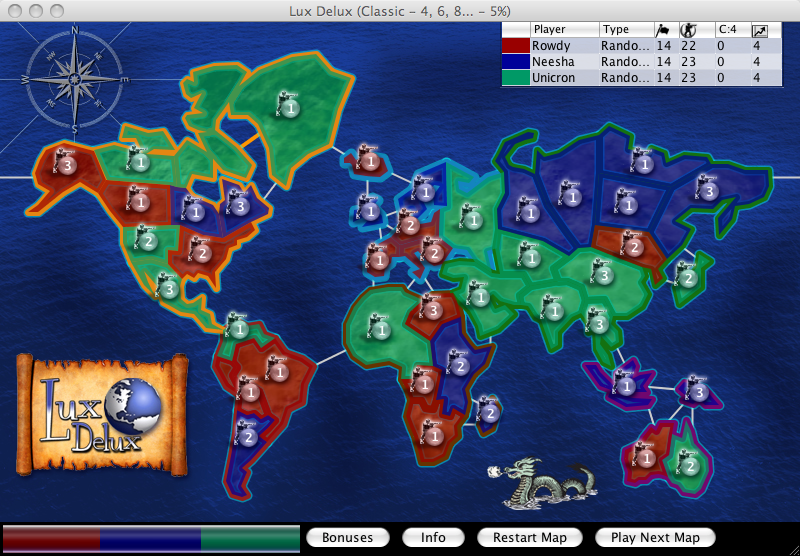
\includegraphics[scale=0.3]{testmap2.png}
%%\caption{Example random draft selection.}\label{fig:random}
%%\end{figure}
%%
%%\begin{figure}[htp]
%%\centering
%%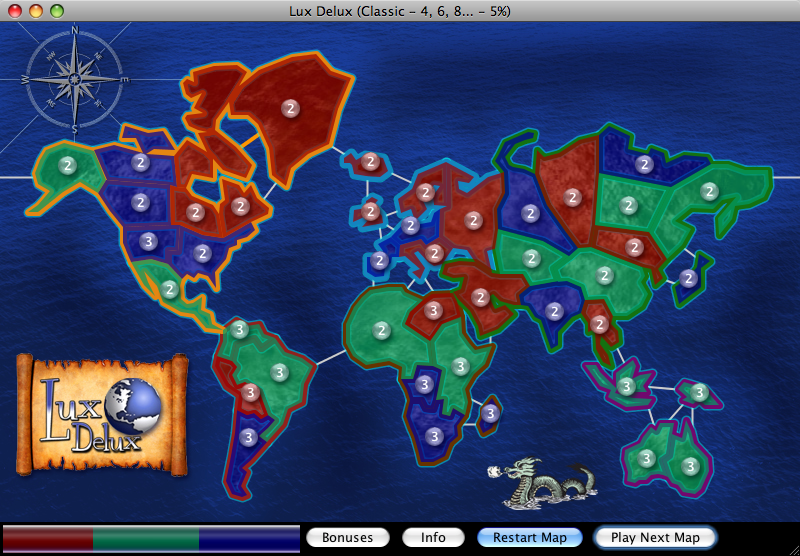
\includegraphics[scale=0.3]{testmapcontinent.png}
%%\caption{Draft selection so that a single player owns a whole continent.}\label{fig:continent}
%%\end{figure}
%
%\begin{table}[]
%%\begin{center}
%%\centering      % used for centering table 
%\begin{tabular}{l l r r r}  % centered columns (5 columns) 
%\hline                       %inserts double horizontal lines
%Draft &  & 0 & 1 & 2 \\[0.5ex]% inserts
%\hline                    % inserts single horizontal line
%0&Evaluation Function&0.278&0.345&0.377\\&Ordered&283&360&357\\&Unordered&420&304&276\\1&Evaluation Function&0.317&0.343&0.34\\&Ordered&322&272&406\\&Unordered&258&309&433\\2&Evaluation Function&0.347&0.342&0.312\\&Ordered&412&354&234\\&Unordered&373&342&285\\3&Evaluation Function&0.323&0.361&0.306\\&Ordered&293&368&339\\&Unordered&347&287&366\\4&Evaluation Function&0.288&0.333&0.379\\&Ordered&330&374&296\\&Unordered&356&368&276\\5&Evaluation Function&0.362&0.302&0.336\\&Ordered&405&356&239\\&Unordered&317&332&351\\6&Evaluation Function&0.195&0.231&0.573\\&Ordered&216&271&513\\&Unordered&247&199&554\\
%[1ex]
%\hline     %inserts single line 
%\end{tabular} 
%%\label{table:nonlin}  % is used to refer this table in the text 
%%\end{center}
%\caption{\label{tab:results} Results of evaluation function and sets on the draft configurations.}
%\end{table}
%
%
%\subsection{Evaluating MaxN-MC using Evaluation Function}
%
%We have run experiments to get an idea of the effectiveness of MaxN-MC using our new evaluation function.  The experiments are set up to have three players.  All three players have identical post-draft strategies provided by a hard-coded Lux agent (namely EvilPixie).  The difference is in the strategies employed in the drafting stage.  While Players 1 and 2 use the hard-coded rules of EvilPixie, Player 0 uses MaxN-MC with our new evaluation function.  Six sets of experiments were run on the world map, each set consisting of 63 to 241 episodes.  An episode is defined as a complete game where each player used their own strategy in the drafting stage then played until a winner is emerged.  
%
%The results are presented in Table~\ref{tab:experiments}.  MAX\_NODES represents the depth in MaxN search where Monte Carlo roll outs take over. NUM\_ROLL\_OUTS represents the number of Monte Carlo roll outs that we average over in MaxN-MC, for each leaf node of the MaxN portion of the search.  A different number of episodes were run for each set of experiments because we have constrained each set to a 24-hour period, and having a larger MAX\_NODES or a larger NUM\_ROLL\_OUTS means that each episode will take longer time.  All experiments show promising results that Player 0 has won a higher number of episodes than the other two players.  Because these results are still preliminary, no conclusions can yet be made.
%
%\begin{table*}[]
%\begin{tabular}{r r r r r r}  % centered columns (6 columns) 
%\hline                       %inserts double horizontal lines
%MAX\_NODES&NUM\_ROLL\_OUTS&Total episodes&Player 0 winning rate&Player 1 winning rate&Player 2 winning rate\\[0.5ex]% inserts
%\hline                    % inserts single horizontal line
%1000&10&190&0.468&0.274&0.258\\
%5000&10&216&0.384&0.361&0.255\\
%10000&10&134&0.425&0.291&0.284\\
%100&100&241&0.432&0.266&0.303\\
%500&100&156&0.423&0.346&0.231\\
%1000&100&63&0.460&0.206&0.333\\
%[1ex]
%\hline     %inserts single line 
%\end{tabular} 
%%\label{table:nonlin}  % is used to refer this table in the text 
%%\end{center}
%\caption{\label{tab:experiments} Results of experiments comparing drafting strategies of MaxN-MC with EvilPixie.}
%\end{table*}

\section{Discussion}

% Discuss our results, what was interesting, what ideas could carry over to drafting games in general

Our experiments in Fantasy Risk indicate that UCT and KthBestPick are our best strategies for this game.  While we did run preliminary experiments that indicated an exploration parameter of $C = 0.01$ worked well with 3000 UCT simulations, we did not do the same in the KthBestPick runs where UCT was able to run many more simulations in the time limit.  It may be the case that with more simulations, higher exploration is beneficial, and so further tests should be run before we can conclude that KthBestPick is superior.  In addition, it would be interesting to see how often KthBestPick is deviating from the top ranked pick provided by UCT simulations; unfortunately, we did not have time to reproduce our experiments to gather this and related statistics.  Finally, we believe that KthBestPick did not benefit by having ``oracle'' opponent models due to similarities in strategies, particularly between UCT and KthBestPick.  Again, statistical evidence of this is needed.

In actual games of Risk, our UCT-Quo bot stands ahead of its competition.  When viewing UCT-Quo in action during the draft, it tends to favour territories in North America, while Quo prefers Australia and South America.  In addition, UCT-Quo is often seen preventing an opponent from owning an entire continent by selecting the last territory remaining in the continent.  However, we cannot take all the credit for the high number of victories as we chose Quo for our post-draft play based on its superior winning percentage against the other three difficult bots in preliminary experiments.  Furthermore, two players following our UCT strategy tend to get in each other's way.  For instance, two UCT-Quos will not let each other claim all of North America since they both believe it to be too valuable.  All the while, the other player is able to gather an entire continent or two which may not appear too strong in the eyes of our imperfect reward signal, but ends up proving to be strong picks nonetheless.  We believe this explains the poor performance of the UCT-Quos in Figure \ref{fig:UCTvsUCTvsQUO}.

\begin{figure}[t]
\centering
\subfigure[]{
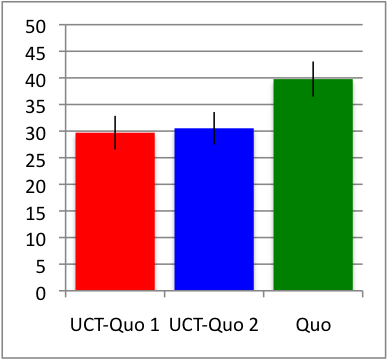
\includegraphics[scale=.55]{figs/2uct.png}
\label{fig:UCTvsUCTvsQUO}
}\hspace{5pt}
\subfigure[]{
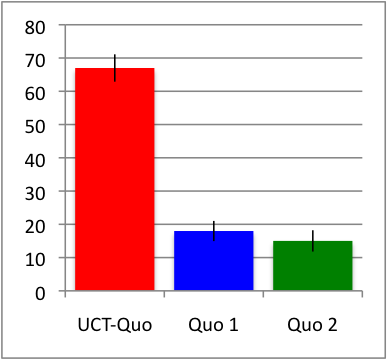
\includegraphics[scale=.55]{figs/2quo.png}
\label{fig:UCTvsQUOvsQUO}
}\hspace{5pt}
\subfigure[]{
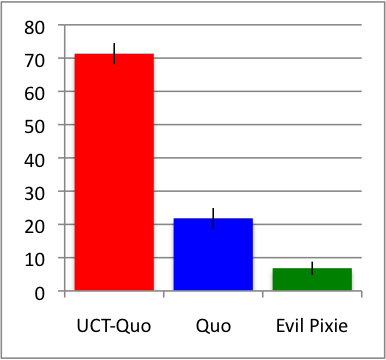
\includegraphics[scale=.55]{figs/evilpixie.png}
\label{fig:UCTvsQUOvsEP}
}\hspace{5pt}
\subfigure[]{
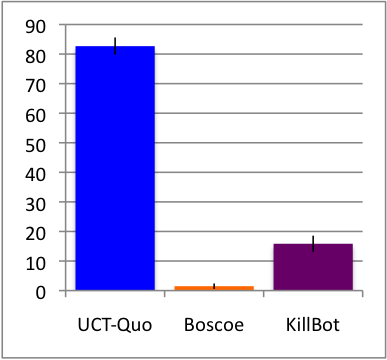
\includegraphics[scale=.55]{figs/others.png}
\label{fig:UCTvsKILvsBOS}
}
\caption[]{Winning percentages in Risk games involving \subref{fig:UCTvsUCTvsQUO}: UCT-Quo vs.~UCT-Quo vs.~Quo, \subref{fig:UCTvsQUOvsQUO}: UCT-Quo vs.~Quo vs.~Quo,  \subref{fig:UCTvsQUOvsEP} UCT-Quo vs.~Quo vs.~Evil Pixie, and \subref{fig:UCTvsKILvsBOS}: UCT-Quo vs.~Boscoe vs.~Killbot.}
\label{fig:ActualRisk}
\end{figure}

% Discuss the strengths (and possibly weaknesses) of the approaches.

\section{Conclusions}

% Summarize 

We formally introduced the concept of a drafting game and shown how to use supervised machine learning to create a reward signal for the drafting sub-game of Risk.  We discussed three strategies, RL, UCT, and KthBestPick, for playing drafting games and tested out each in Fantasy Risk, our abbreviated Risk game.  The strongest players in Fantasy Risk were KthBestPick and UCT, and our augmented UCT-Quo bot performed exceptionally well in actual Risk games.

%This paper has formalized the concept of a drafting game.    We introduced two solutions for playing a drafting game.  Our first approach, MaxN-MC, is a combination of the MaxN algorithm, which generalizes minimax search to multi-player games, and Monte-Carlo simulations, as used in Monte-Carlo tree search algorithms.  Our second technique is KthBestPick, which uses heuristics to rank actions and opponent models to predict which actions will be selected by other players.  

We conclude by listing some possible avenues of further research:
\begin{itemize}
	\item determine how to model opponents on-line in Fantasy Risk to learn opponent models for KthBestPick.
	\item apply our techniques to other drafting games, such as drafting in fantasy sports.  KthBestPick may perform even better in domains where an obvious heuristic exists, such as in the drafting game depicted in Table \ref{tab:KthEx}.  In fantasy sports, actions are usually grouped into types (eg.~a hockey player's position) where each player must select a certain number of actions of each type.  A numerical value (additive reward) is typically associated with each action (eg.~picking a hockey player) estimating the number of points that pick will provide to the fantasy team.  This value provides a simple heuristic for KthBestPick without the need for another algorithm such as UCT.  KthBestPick can then spend all of its efforts determining which of the highest ranked picks to make depending on the number of picks already made of each type by all the players.
	\item use a more sophisticated system for engineering a reward signal, such as an artificial neural network.  This may alleviate the poor performance of UCT-Quo in Figure \ref{fig:UCTvsUCTvsQUO}, and would provide a new, likely more complex drafting game to compare algorithms against than our current game of Fantasy Risk.
	\item find improvements to our RL methods for drafting.
%	\item use opponent modelling within UCT.
\end{itemize}

\section*{Acknowledgments}
We would like to thank Vadim Bulitko for directing us to Lee's thesis and for suggesting Fantasy Risk.  %We would also like to thank SillySoft for providing full source code of their Risk bots in Lux Delux.

%\bibliography{../../../LaTeX/bib}
%\bibliographystyle{../../../LaTeX/Styles/aaai}
\bibliography{bib}
\bibliographystyle{aaai}

\end{document}
